\section{Introduction} \label{man-introduction}
This section will go in detail about the working of the system.
We created an application that is able to generate a RSA encryption.

\section{Application} \label{man-application}
This section will provide information about the setup of the program.
Make sure there are no spaces in the input. This will trip the application.

Be also aware that the calculation of P and  Q could take a time based on the N.
This is also applicable to decryption because P and Q aren't know if E and N is provided. This is way it takes a time to decrypt. 
\subsection{Run}
The application can be run by clicking the application.

\subsection{RSA}
The program differs from an original RSA structure. This is thanks the the input N that will generate the P and Q.

The rsa object has multiple variables that will be shown below.

The note worthy variables are INIT\_NUMBER, this will init the first prime that will be used to calculate P and Q.

\begin{lstlisting}{}
private Random rand = new Random();
public static final BigInteger INIT_NUMBER = new BigInteger("2");
private final static BigInteger one = new BigInteger("1");
private String calculateTime;
private BigInteger p, q, n, e, d, phi;
\end{lstlisting}

We choose to use Big Interger for the provided methods that come with the Math package.
Such methods are modPow, probablePrime and isProbablePrime.

To generate P and Q we use te method calculatePAndQ based on the input N.

\begin{lstlisting}
public void calculatePandQ(String nInput) {
    this.n = new BigInteger(nInput);
    long begin = System.currentTimeMillis();
    //Initialise n and p
    BigInteger p = INIT_NUMBER;
    //For each prime p
    while (p.compareTo(n.divide(INIT_NUMBER)) <= 0) {
        //If we find p
        if (n.mod(p).equals(BigInteger.ZERO)) {
            //Calculate q
            BigInteger q = n.divide(p);
            //Displays the result
            this.p = p;
            this.q = q;
            calculateTime = String.valueOf(System.currentTimeMillis() - begin);
            //The end of the algorithm
            return;
        }
        //p = the next prime number
        p = p.nextProbablePrime();
    }
    calculateTime = "No solution exists";
}
\end{lstlisting}

With those steps P and q are generated.

\section{Generate E}
To generate E we first calculate phi, then we loop and generate an E till E  < phi and co-prime to phi.

The code looks as following
\begin{lstlisting}  
phi = p.subtract(one).multiply(q.subtract(one));
do {
    e = new BigInteger(phi.bitLength(), rand);
} while (e.compareTo(one) <= 0 || e.compareTo(phi) >= 0 || !e.gcd(phi).equals(one));
d = e.modInverse(phi);
\end{lstlisting}{}

\section{encryption}
To encrypt the message we first split the string in a char array.
Every char will be cast to an integer value and that value will be encrypted.
The cipherText will splitt each char with a ,.

\begin{lstlisting}
String cipherText = "";
ArrayList<Integer> convert = convertString(message);
for(Integer i : convert){
    cipherText =cipherText + BigInteger.valueOf(i).modPow(e, n) + ",";
}
System.out.println(d + "    =d---e=     " + e + "----- n = " + n);
return cipherText;
\end{lstlisting}{}


\section{Decryption}
To Decode we will handle input e and N and calculate P and q based on input.
Then D will be calculated with the provided input and the calculated P and Q.

\begin{lstlisting}
e = new BigInteger(inputE);
calculatePandQ(inputN);
d = e.modInverse(phi);
\end{lstlisting}{}

\subsection{Step 2}
In the first step we will generate a private key, in the final step we will use this private key to decode the cipher.

Finally every char will BigInteger will be cast to a int that will translate to the message.

By making use of the stream method we can convert the whole array to the original message.

\begin{lstlisting}
public String decodeCipher(String cipherText) {
    String[] cipherArray = cipherText.split(",");
    ArrayList<Character> mess = new ArrayList<>();
    for(String c : cipherArray){
        BigInteger letter = new BigInteger(c).modPow(d, n);
        mess.add((char)letter.intValue());
    }
    return  mess.stream().map(e->e.toString()).reduce((acc, e) -> acc  + e).get();
}
\end{lstlisting}

\section{Examples}
\begin{figure}
    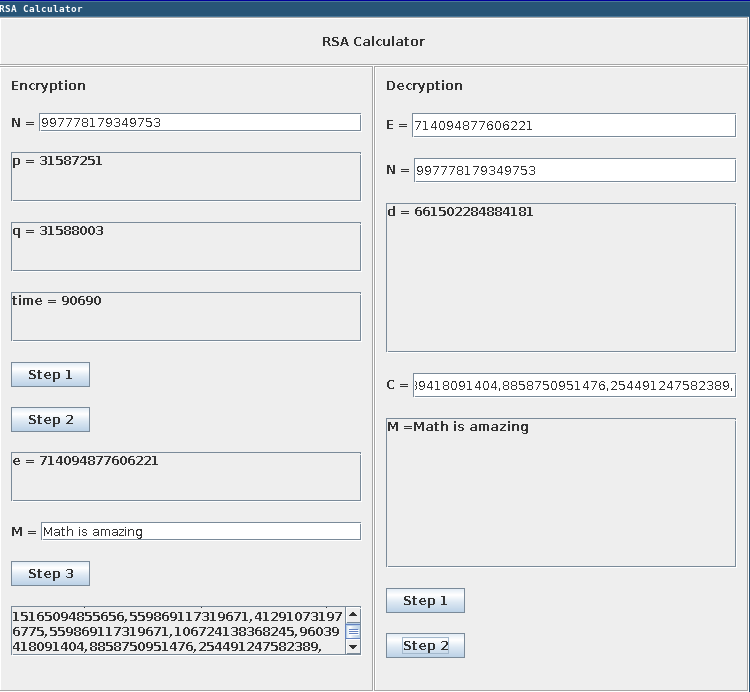
\includegraphics[width=\linewidth]{images/example_1}
    \caption{example 1}
    \label{fig:boat1}
\end{figure}
